% !TEX root = ../thesis.tex

\chapter{Mikrosvety vo výučbe programovania}

In the 1960s, the late Seymour Papert
and his colleagues at MIT developed
the Project LOGO turtle and began
using it to teach schoolchildren how
to program.
• The LOGO turtle was one of the first
examples of a microworld, a simple,
s~e l f - c o~n t a i n e d p r o~g r a m m i n g
environment designed for teaching.
• Papert described his experiences and
his theories about education in his
book Mindstorms, which remains one
of the most important books about
computer science pedagogy.

\emph{Mikrosvet} predstavuje malú, ale úplnú reprezentáciu vybranej domény \cite{bertz} \cite{Rieber1996}.

V~nasledujúcich podkapitolách sa nachádza prehľad niektorých známych mikrosvetov v~našom regióne. Mikrosvet \emph{Robota Karla} bude predstavený v~nasledujúcej kapitole.



\section{Korytnačia grafika}

jazyk LOGO

\section{Baltík}





\chapter{(Mikro)svet Robota Karla}

Do mikrosvetov, ktoré sú určené na výučbu programovania, patrí aj \emph{Robot Karel}. Imperatívny jazyk \emph{Robota Karla} navrhol v~roku 1970 postgraduálny študent \emph{Stanfordskej univerzity} \emph{Richard Pattis}. \emph{Richard} sa rozhodol, že študenti sa jednoduchšie naučia základy programovania, ak sa ich budú učiť v~jednoduchom prostredí bez zbytočných komplexností, ktoré sú charakteristické pre väčšinu programovacích jazykov.\cite{karel_learns_java}

\begin{figure}[htbp]
    \centering
    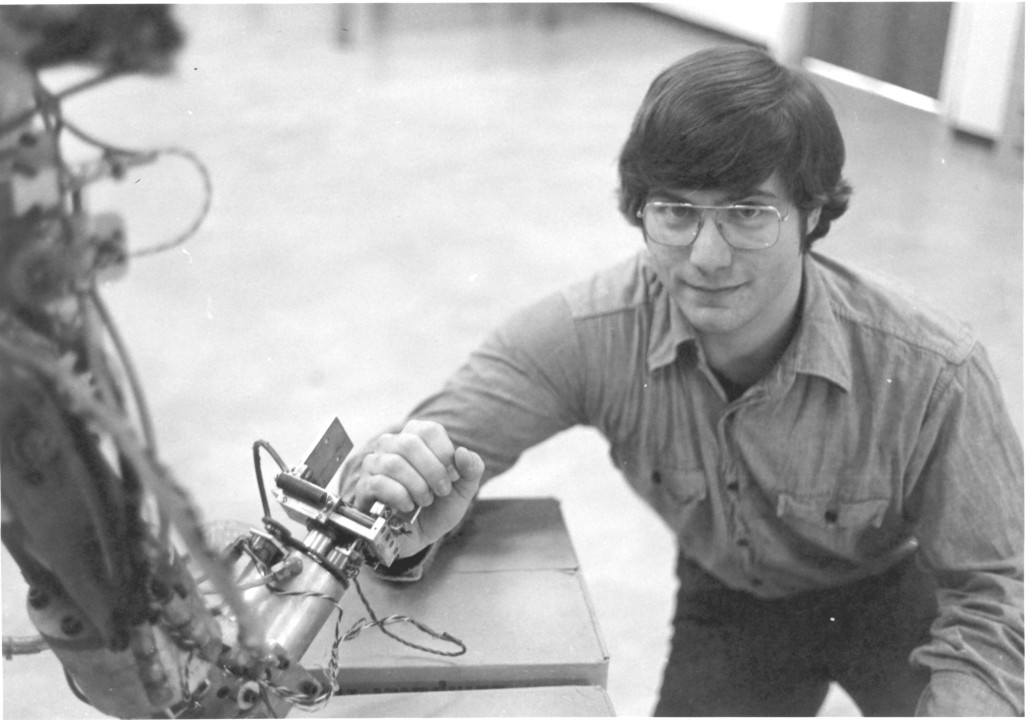
\includegraphics[width=.9\textwidth]{figures/richard.pattis.jpg}
    \caption[Richard Pattis]{Richard Pattis \footnotemark }
\end{figure}

\footnotetext{Zdroj: \url{https://www.cs.cmu.edu/~pattis/}}

Meno robota \emph{Pattis} vybral podľa českého autora \emph{Karla Čapka}, ktorý v~roku 1921 napísal divadelnú hru s~názvom \emph{R.U.R.}, v~ktorej bolo meno \emph{robot} prvýkrát použité.

V~roku 1981 \emph{Pattis} vydal knihu s~názvom \emph{Karel the
Robot: A~Gentle Introduction to the Art of Programming} \cite{Pattis1994}, ktorá sa stala veľmi populárnou učebniciou tohto jazyka.



\section{asdf}

z~coho sa svet robota karla sklada

steny, znacky

streets (ulice, riadky) a avenues (aleje, stlpce)

\section{Primitívy a senzory Robota Karla}

\section{Robot Karel a objektové programovanie}

Aj keď bol pôvodne programovací jazyk \emph{Robot Karel} navrhnutý pre výučbu procedurálneho programovania, vznikli rôzne implementácie aj pre výučbu objektového programovania. Napríklad aj samotní autori pôvodnej učebnice vydali knihu s~názvom \emph{Karel++: A~Gentle Introduction to the Art of Object-Oriented Programming} \cite{Pattis1996}, ktorá sa venuje práve objektovému programovaniu s~\emph{Robotom Karlom} v~jazyku \emph{C++}. Samozrejme sa dá stretnúť s~rozličnými implementáciami v~mnohých súčasných programovacích jazykoch, ktoré poskytujú objektovú paradigmu.


\lstinputlisting[caption={Ukážka programu v~pôvodnom jazyku podľa \cite{Pattis1994}}]{listings/program.karel}

\section{Robot Karel v~Československu}

V 80-tych rokoch minulého storočia bol \emph{Robot Karel} veľmi populárny aj v Československu. Za svoju popularitu vďačí najmä 3D verzii pre 8-bitové mikropočítače \emph{PMD 85}, za ktorou stojí \emph{Marián Vittek} z \emph{Univerzity Komenského v Bratislave}.

\begin{figure}[!ht]
    \centering
    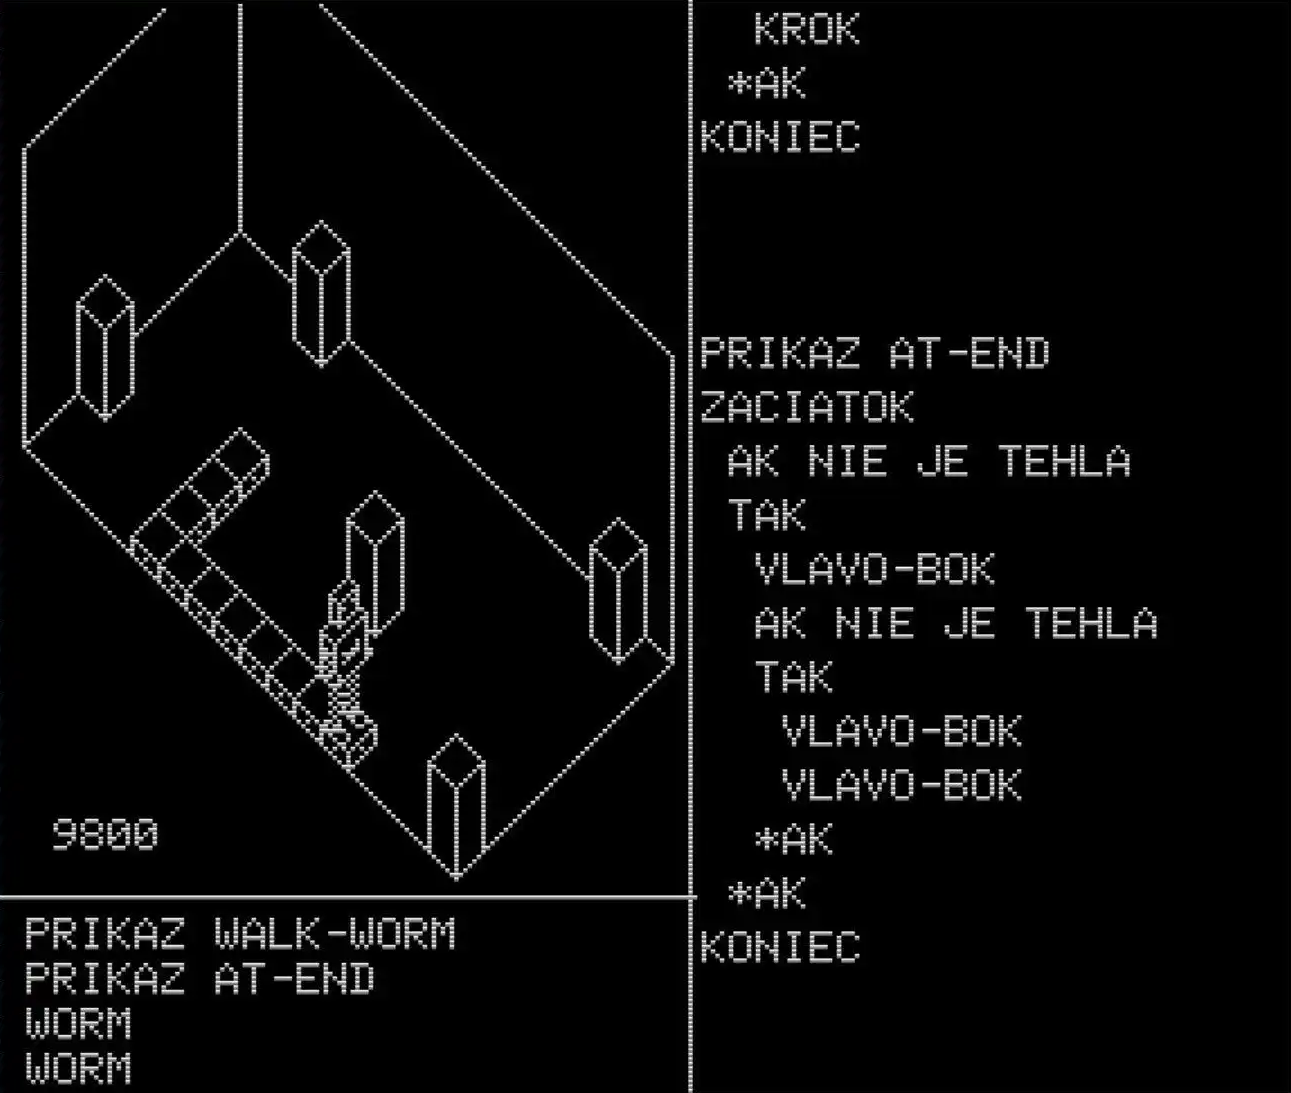
\includegraphics[width=.9\textwidth]{figures/karel3d.png}
    \caption{Robot Karel v~3D na mikropočítači PMD 85}
\end{figure}

Podpore programovacieho jazyka \emph{Karel} sa venoval aj časopis \emph{Zenit pionierov} (slovenská obdoba českého časopisu \emph{ABC}), kde mu v istom čase bola venovaná jedna strana v seriáli \emph{Kamarát Karel}. V čísle 25 ročníka 1987-88 sa dokonca \emph{Robot Karel} objavil aj v podobe vystrihovačky.

\begin{figure}[!ht]
    \centering
    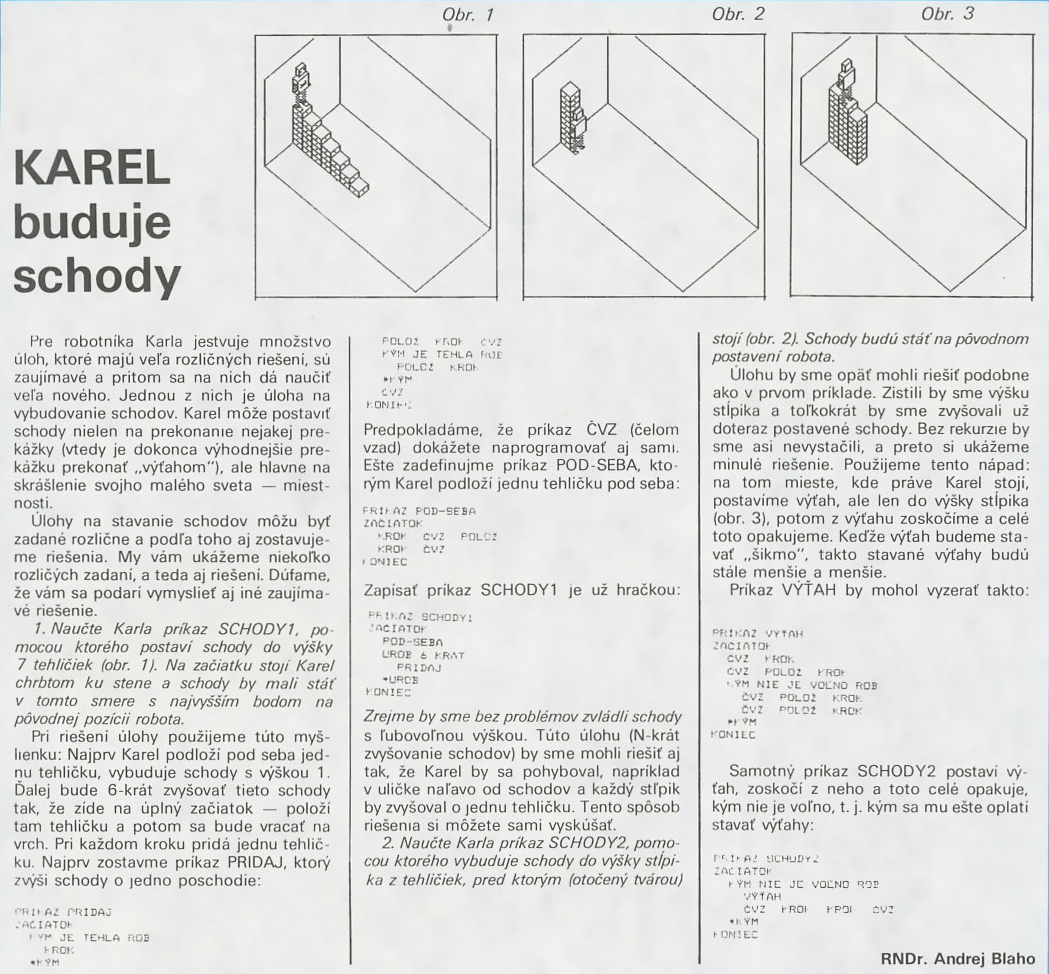
\includegraphics[width=.9\textwidth]{figures/karel.v.zenite.pionierov.png}
    \caption{Jedna z častí seriálu \emph{Kamarát Karel} v časopise \emph{Zenit pionierov}}
\end{figure}

\emph{Robotovi Karlovi} boli venované aj niektoré knihy. Napríklad kniha \emph{Martina si hraje s počítačem} \cite{Synovcova1989} z roku 1989 obsahovala 107 programov pre \emph{Robota Karla} a spolu s nimi aj vystrihovačku, vďaka ktorej mohli prograomvať aj tí, ktorí prístup ku mikropočítaču nemajú.

V roku 1991 zasa vyšla kniha \emph{Kamaráti robota Karla} \cite{Gasparovicova1991}, ktorá však už bola určená pre PC verziu \emph{Robota Karla}.

Pre rozličné platformy a architektúry vznikli v Československu a neskôr v Českej republiku a na Slovensku rôzne implementácie, ktoré vznikajú dodnes. Najznámejším projektom v súčasnosti by mohol byť \emph{Robot Emil} z projektu \emph{Informatika s Emilom}\footnote{\url{https://www.robotemil.com/}}.

\emph{Robot Karel} býva taktiež témou záverečných prác na univerzitách v Čechách a na Slovensku, čoho dôkazom je aj táto práca.



